\documentclass[11pt,letterpaper]{article}
\usepackage[T1]{fontenc}\usepackage[utf8]{inputenc}\usepackage{lmodern}\usepackage{microtype}
\usepackage[margin=1in]{geometry}\usepackage{graphicx,booktabs,array,amsmath,amssymb}
\usepackage{textcomp,xcolor,caption,setspace}
\usepackage[numbers,sort&compress]{natbib}\usepackage[hidelinks]{hyperref}
\ifdefined\reviewmode\usepackage{lineno}\linenumbers\setstretch{1.3}\fi
\captionsetup{font=small,labelfont=bf,justification=raggedright,singlelinecheck=false}
\renewcommand{\arraystretch}{1.12}\setlength{\tabcolsep}{4pt}
\setlength{\emergencystretch}{2em}\setlength{\textfloatsep}{14pt plus 2pt minus 2pt}
\newcommand{\SpO}{SpO\textsubscript{2}}
\newcommand{\tightnote}[1]{\par\smallskip{\footnotesize\raggedright #1\par}}
\title{\bfseries Alarm burden beyond threshold replay:\\linked-reward calibration of recorded clinical alarms}
\author{
Zihao Wang$^{1}$, Michele Ceccarelli$^{1,2,\dagger}$, Min Lu$^{1,\dagger,\ast}$\\[2pt]
\small $^{1}$Division of Biostatistics \& Bioinformatics, Department of Public Health Sciences,\\
\small Miller School of Medicine, University of Miami, Miami, FL, USA\\
\small $^{2}$Sylvester Comprehensive Cancer Center, University of Miami Miller School of Medicine,
Miami, FL, USA\\[2pt]
\small $^{\dagger}$These authors contributed equally and jointly supervised this work.\\
\small $^{\ast}$Correspondence:
Michele Ceccarelli (\texttt{mxc2982@miami.edu}),
Min Lu (\texttt{m.lu6@umiami.edu})
}
\date{}
% ---- inlined from 01_main/figures_main.tex ----
\newcommand{\figalt}[1]{\par\smallskip{\footnotesize\raggedright\textit{Alt text:} #1\par}}
\newcommand{\placefig}[1]{#1}
\newcommand{\placetab}[1]{#1}
\newcommand{\TabSimulation}{
% ---- inlined from 01_main/TAB_SIMULATION_MAIN.tex ----
\begin{table}[htbp]\centering\small
\caption{Simulation performance for the principal estimator and comparators in selected scenarios from Table~\ref{tab:simdesign}.}
\label{tab:sim}
\begin{tabular}{@{}llrrr@{}}\toprule
Scenario & Method & Bias & RMSE & Coverage\\\midrule
A: Transport holds & Replay & -8.07 & 8.13 & ---\\
 & Duration-only & -0.09 & 1.34 & 0.935\\
 & Feature-augmented & -0.08 & 1.34 & 0.935\\
\addlinespace
D: Overshoot and composition shift & Replay & -16.35 & 16.38 & ---\\
 & Duration-only & -8.37 & 8.47 & 0.000\\
 & Feature-augmented & -0.06 & 1.25 & 0.945\\
\addlinespace
G: Feature-dependent zero inflation & Replay & -13.50 & 13.54 & ---\\
 & Duration-only & -3.92 & 4.18 & 0.195\\
 & Feature-augmented & -0.15 & 1.43 & 0.915\\
\addlinespace
H: Incomplete support & Replay & 17.53 & 17.62 & ---\\
 & Duration-only & 11.75 & 12.03 & 0.010\\
 & Feature-augmented & 11.76 & 12.03 & 0.010\\
\addlinespace
I: Reward transport fails & Replay & -22.35 & 22.37 & ---\\
 & Duration-only & -14.37 & 14.43 & 0.000\\
 & Feature-augmented & -14.36 & 14.42 & 0.000\\
\addlinespace
\bottomrule\end{tabular}
\tightnote{Bias and root mean squared error (RMSE) are percentage points for the true linked-burden reduction. Each scenario uses 300 patients and 500 replicates; coverage uses the first 400 replicates and 200 patient bootstrap resamples. The feature map is selected on an independent sample. Nominal coverage is 0.95. Replay has no interval. Incomplete support and transport failure deliberately violate identification assumptions; the intervals are not expected to cover the scientific target in these settings. Complete Monte Carlo diagnostics and additional scenarios are in the supplement.}
\end{table}

% ---- end inline ----
}
\newcommand{\TabPolicy}{
% ---- inlined from 01_main/TABLE_POLICY.tex ----
\begin{table}[!htbp]\centering\small
\caption{Interpretation diagnostics for a one-step less stringent limit.}
\label{tab:policy}
\begin{tabular}{@{}lrrrr@{}}\toprule
 & \multicolumn{1}{c}{Unlinked} & \multicolumn{1}{c}{Unobserved} & \multicolumn{1}{c}{Coarsened} & \multicolumn{1}{c}{Pooled-tail}\\
Channel & \multicolumn{1}{c}{recorded share} & \multicolumn{1}{c}{fine-cell share} & \multicolumn{1}{c}{linked share} & \multicolumn{1}{c}{replay share}\\\midrule
Respiration rate, low & 9\% & 0.07\% & 0.5\% & 5.6\%\\
\SpO{}, low & 13\% & 0.03\% & 0.5\% & 20.4\%\\
Heart rate, high & 14\% & 0.16\% & 9.2\% & 19.3\%\\
Heart rate, low & 25\% & 2.65\% & 21.0\% & 32.3\%\\\bottomrule
\end{tabular}
\tightnote{Unlinked recorded share is baseline recorded alarm time assigned to no excursion. Unobserved fine-cell share is candidate replayed time in duration--overshoot cells with no baseline excursion. Coarsened linked share is estimated candidate linked burden assigned a parent duration rate under the independent tuning map. Pooled-tail replay share is candidate replayed time in bins at or above 120 seconds. Different denominators are intentional. These diagnostics do not convert a coarsened estimate into fully identified feature-specific transport.}
\end{table}

% ---- end inline ----
}
\newcommand{\TabSimDesign}{
% ---- inlined from 01_main/TABLE_SIMDESIGN.tex ----
\begin{table}[htbp]\centering\small
\caption{Simulation scenarios. All scenarios share the excursion law of Section~\ref{sec:sim}; the second column states what differs from A.}
\label{tab:simdesign}
\begin{tabular}{@{}l>{\raggedright\arraybackslash}p{6.7cm}>{\raggedright\arraybackslash}p{7.2cm}r@{}}\toprule
 & Departure from the reference law & Condition examined & Patients\\\midrule
A & None: reward $0.85(d-8)_+$ at both limits, no overshoot dependence; the candidate shortens excursions (duration scale 14 to 11) and leaves the overshoot composition unchanged & Duration transport (T-d) and joint transport (T) both hold; replay understates the reduction under the stated monotone reward pattern & 300\\
B & Patient-effect shape $k=1.2$ in place of $4$ & Heavier-tailed patient effects and more unequal excursion counts, testing patient-cluster bootstrap inference & 300\\
C & Reward multiplier rises with duration, $\min\{0.95,\,0.55+0.004d\}$ & Reward heterogeneity within the pooled duration cells & 300\\
\addlinespace
D & Reward multiplier $(0.45,0.70,0.85,0.92)$ by overshoot class; candidate composition $(0.25,0.30,0.25,0.20)$ to $(0.45,0.28,0.17,0.10)$ & Duration transport fails while joint transport holds & 300\\
E & As D & Sparse feature cells: map selection and coarsening with few excursions per cell & 60\\
\addlinespace
F & Non-annunciation with probability $p(d)=0.40\{0.20+0.80\,e^{-(d-2)/30}\}$; composition shifts as in D & Observed zeros at every duration; duration transport still holds & 300\\
G & As F, with the class multipliers $(0.65,0.45,0.25,0.12)$ in place of $0.40$ & Zeros that depend on overshoot, so that joint transport is needed & 300\\
\addlinespace
H & Baseline durations capped at 100\,s, a point mass there; the candidate lengthens excursions (duration scale 20) & Overlap fails: candidate cells occur with no baseline excursion, violating the support condition required for calibration & 300\\
I & Candidate reward multiplied by $0.8$ & Reward transport fails under either specification & 300\\
\bottomrule\end{tabular}
\tightnote{Patient effects $F_i$ are Gamma with shape $k$ divided by $k$; excursion counts are $\max\{1,\mathrm{Poisson}(25F_i)\}$; durations are Gamma with shape 1.6 and scale $s_uF_i^{0.3}$, rounded up to the two-second grid; overshoot classes $z=0,\dots,3$; positive rewards are Gamma with mean $m(d,z)$ and scale 3, and excursions at or below the 8-second persistence clock earn zero. The full specification is in the supplement.}
\end{table}

% ---- end inline ----
}
\newcommand{\FigSimulation}{\begin{figure}[htbp]\centering
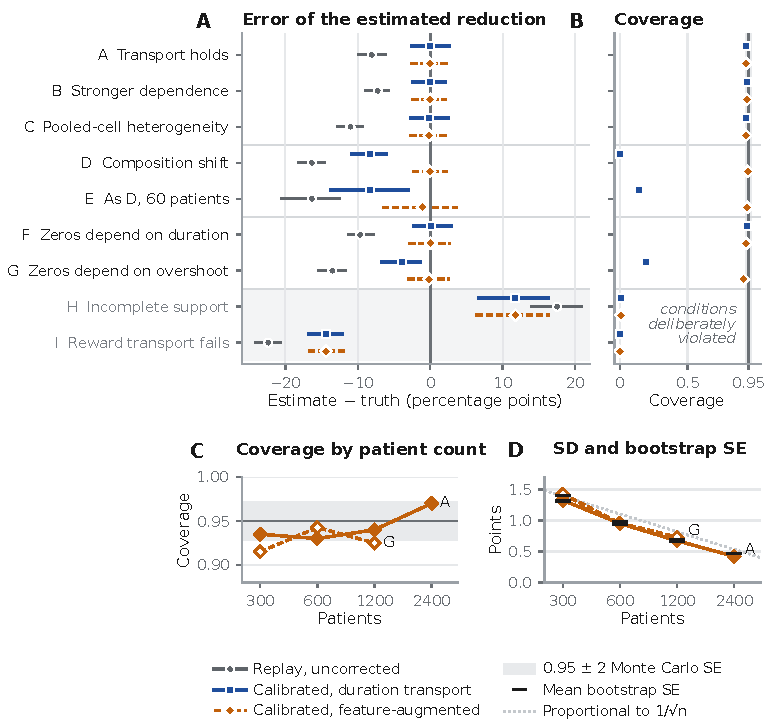
\includegraphics[width=\textwidth]{figures/Figure2_simulation.pdf}
\caption{Simulation summary for the nine scenarios of Table~\ref{tab:simdesign}. A: estimate minus truth, in percentage points of the linked-burden reduction, for uncorrected replay and the two calibrated estimators; the mark is the replicate mean and the line spans the central 95\% of the 500 replicate errors. The shaded rows deliberately violate an identification condition. B: coverage of the 95\% patient-cluster bootstrap intervals over 400 replicates; the band is $0.95$ plus or minus two binomial Monte Carlo standard errors. C and D: the feature-augmented estimator as the patient count grows in scenarios A and G: coverage, and the empirical standard deviation beside the mean bootstrap standard error, against a reference proportional to $n^{-1/2}$.}
\label{fig:simulation}
\figalt{Four panels. In the first, replay is biased in every scenario, from about minus 22 to plus 18 points, while the calibrated estimators are centred on zero wherever their conditions hold; duration-only calibration is biased when the reward depends on overshoot, and both calibrated estimators are biased, with narrow spread, when support or reward transport fails. In the second, coverage sits near 0.95 in the same scenarios in which the estimators are unbiased and near zero otherwise. The lower panels show coverage between 0.915 and 0.970 as the patient count grows from 300 to 2,400, and an empirical standard deviation that falls in proportion to one over the square root of the patient count, with the mean bootstrap standard error alongside it.}
\end{figure}}
\newcommand{\FigObservation}{\begin{figure}[htbp]\centering
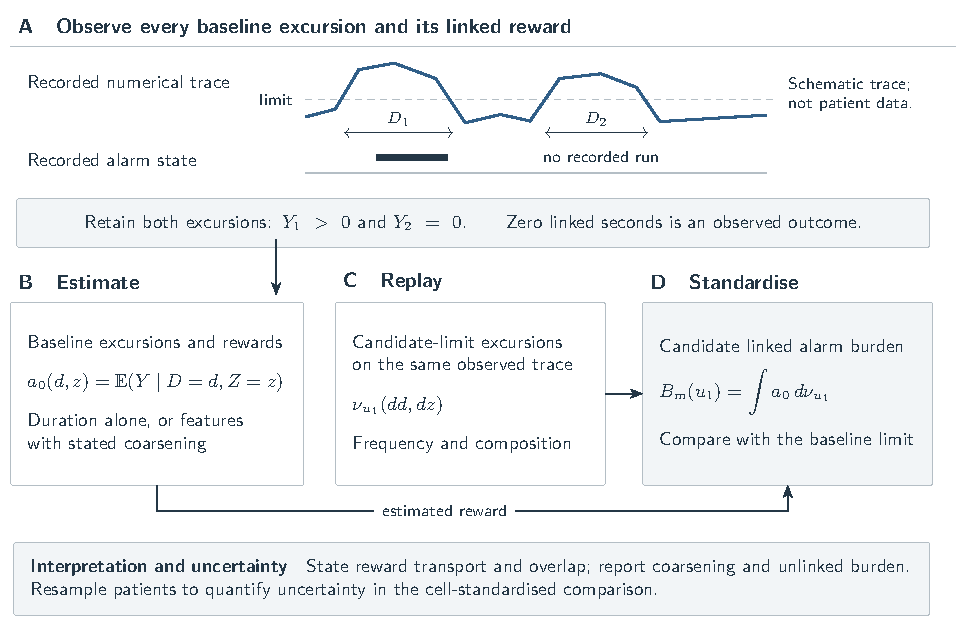
\includegraphics[width=\textwidth]{figures/Figure1_framework.pdf}
\caption{Linked-reward calibration. A baseline excursion is retained whether it has a linked alarm or an observed zero reward. The estimated reward is then standardised over excursions replayed at a candidate limit. The schematic integral shows joint reward transport; duration-only transport and the implemented coarsened cell estimator are described in the text.}
\label{fig:observation}
\figalt{A schematic trace contains two threshold excursions but only one recorded alarm. Both excursions enter estimation, one with positive linked seconds and the other with zero. Subsequent panels show conditional reward estimation, candidate-limit replay and their combination in a standardised linked-burden comparison. A final note distinguishes transport and overlap assumptions from patient-level sampling uncertainty.}
\end{figure}}
\newcommand{\FigHoldout}{\begin{figure}[htbp]\centering
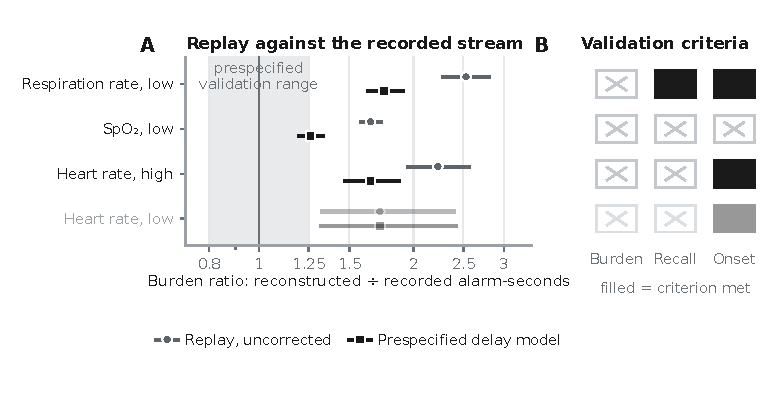
\includegraphics[width=\textwidth]{figures/Figure3_holdout.pdf}
\caption{Held-out validation against recorded annunciations. A: replayed-to-recorded alarm-second ratios with 95\% patient-cluster bootstrap intervals. The shaded validation range was prespecified. B: the delay model's three validation criteria: burden ratio in $[0.80,1.25]$, recall at least $0.90$, and onset agreement within 10 seconds for at least $0.80$ of matched episodes. No channel met all three criteria.}
\label{fig:holdout}
\figalt{Four rows compare uncorrected replay and a prespecified delay model. Uncorrected burden ratios range from 1.65 to 2.53, all above one. The delay model improves three channels but none meets all three validation criteria; the matrix marks individual criteria met or not met.}
\end{figure}}
\newcommand{\FigRewardDuration}{\begin{figure}[p]\centering
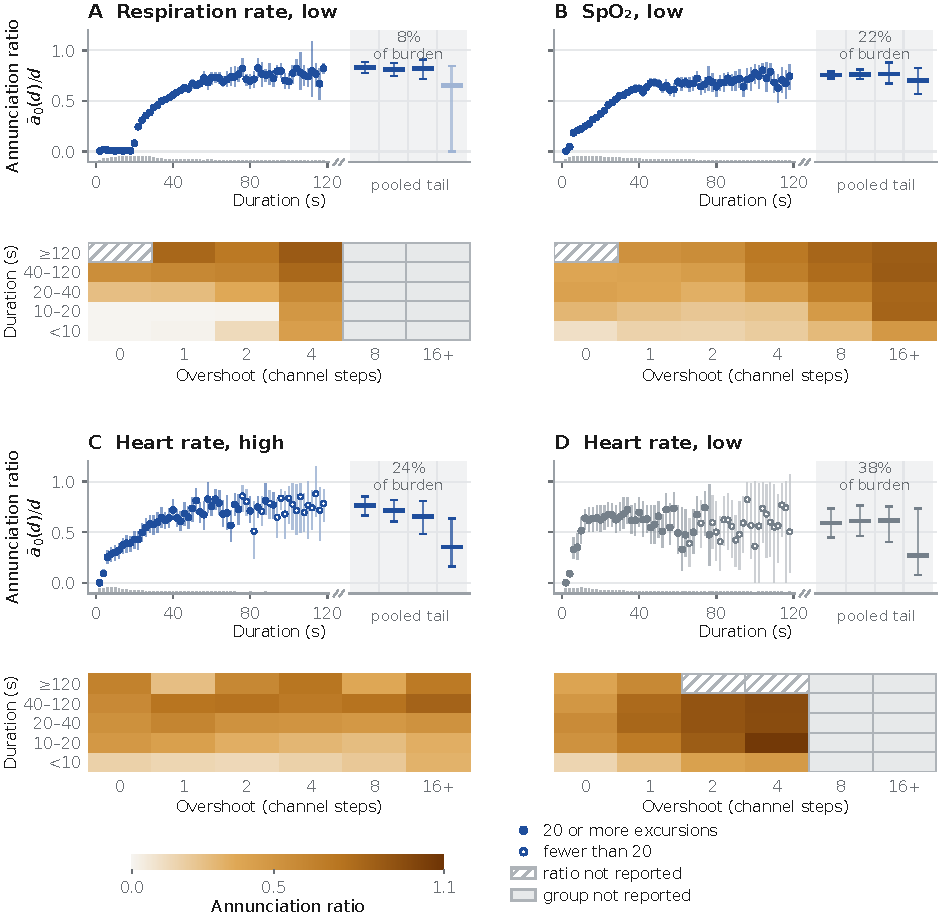
\includegraphics[width=\textwidth]{figures/Figure4_reward.pdf}
\caption{Estimated linked-annunciation reward in four channels. Each panel pairs duration-marginal ratios (upper plot; pointwise 95\% patient-cluster intervals) with ratios by duration and overshoot group (lower plot). Open points mark bins with fewer than 20 excursions. Four equal-width positions after the axis break represent $[120,180)$, $[180,300)$, $[300,600)$ and $[600,\infty)$ seconds; their combined replay-duration share is annotated. Unreported heat-map cells include groups below the export minimum of 30 excursions. This display rule is distinct from the five-excursion rule used to select the feature-estimation map.}
\label{fig:reward}\label{fig:reward_overshoot}
\figalt{Four channel panels show unconnected duration-bin estimates and overshoot heat maps. Ratios are generally higher for longer excursions, but are not pointwise monotone and decline in some pooled tails. Overshoot adds information on respiration-rate low, oxygen-saturation low and heart-rate low; its relationship is weaker and nonmonotone on heart-rate high. The common heat-map scale includes values above one.}
\end{figure}}
\newcommand{\FigPolicy}{\begin{figure}[htbp]\centering
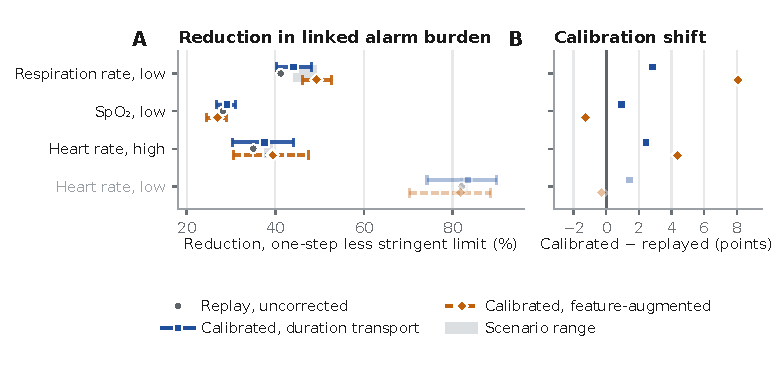
\includegraphics[width=\textwidth]{figures/Figure5_policy.pdf}
\caption{One-step less stringent alarm limits. A: replayed and calibrated reductions, with 95\% patient-cluster intervals for the two cell-standardised estimates. B: calibrated minus replayed reduction in percentage points; these are point estimates, not intervals. The shaded span between the two calibration estimates denotes alternative specifications, not a confidence interval or identified set. The feature-augmented estimate uses duration-only coarsening; this is particularly consequential on heart-rate low, where full joint-feature transport is not identified from the observed fine-cell overlap.}
\label{fig:policy}
\figalt{The absolute reduction ranges from approximately 27 to 84 percent across channels. A separate panel shows smaller calibration shifts, ranging from about minus one to plus eight percentage points. Respiration-rate low has the largest positive shift. Heart-rate low is de-emphasised because substantial coarsening and limited fine-cell overlap restrict its feature-specific interpretation.}
\end{figure}}

% ---- end inline ----

\begin{document}\maketitle
\begin{abstract}\noindent
% ---- inlined from 01_main/_chunks/abstract.tex ----
Retrospective studies estimate how changing bedside-monitor alarm limits would affect alarm burden by replaying thresholds on stored vital-sign measurements. This can mislead, because a threshold excursion is not necessarily annunciated: persistence rules, averaging, signal-quality handling, alarm priority, silencing and inactivation all separate the numerical trace from the alarm stream. We quantified this gap and developed linked-reward calibration, which anchors replay to the alarms a monitor actually recorded. Every replayed excursion is retained, including those with no linked alarm, which contribute zero linked seconds; baseline linked alarm time is then standardised over excursions generated by candidate limits under explicit transport and overlap assumptions. In a two-hospital telemetry database of 12\,241 admissions, held-out replay overestimated recorded alarm seconds by $1.65$--$2.53$-fold across four channels and a prespecified delay correction failed validation. Only 23\%--35\% of replayed excursions carried a linked alarm, while 9\%--25\% of recorded alarm seconds were unlinked. For a one-step less stringent respiration-rate limit, a replayed reduction of 41.2\% became 44.1\% or 49.3\% under two specifications. Threshold crossings, recorded alarms and non-annunciated periods are therefore distinct components of alarm burden, and calibration makes retrospective alarm-limit evaluation more credible where monitor logic is unavailable, while keeping its assumptions and unresolved burden explicit.

% ---- end inline ----
\end{abstract}
\noindent\textbf{Keywords:} alarm burden; alarm management; clinical monitoring; physiological alarms; silencing; threshold replay.
\section{Introduction}\label{sec:intro}
% ---- inlined from 01_main/_chunks/n1_intro.tex ----
Continuous physiological monitoring is central to detecting deterioration, but frequent or nonactionable alerts impose substantial cognitive and workflow burden \citep{chambrin1999multicentric,drew2014insights,cvach2012monitor,bonafide2015association,bonafide2017video,rasooly2021burden,hyland2020circulatory}. Translational monitoring studies increasingly judge alerting systems not only by discrimination but by whether they produce a manageable alert stream that fits real care pathways \citep{henry2015trewscore,hyland2020circulatory,lin2024ecg,rossetti2025concern}. Alarm management therefore turns on limits and persistence requirements that suppress unnecessary annunciations while preserving useful information \citep{ruskin2015alarmfatigue,hravnak2018call,paine2016systematic,winters2018technological}. Retrospective studies usually evaluate such choices by \emph{threshold replay}: applying a proposed limit to stored measurements and summing the resulting excursions \citep{welch2016multiparameter,poole2018personalized,vanrossum2022adaptive}. Replay can compare settings that were never implemented, but interpreting it requires distinguishing a threshold crossing from an alarm the monitor recorded.

Monitors apply persistence requirements, averaging, signal-quality suppression and priority rules, so annunciation can begin after an excursion starts, end before it ends, or persist after the signal returns within range \citep{iec2020alarms,aami2002ec13,imhoff2006algorithms}; changing those rules alters alarm counts and durations substantially \citep{rheineck1998influence,vagedes2014conversion,mcclure2016alarms,gorges2009delays,schmid2017adaptive}. A replayed excursion duration is therefore a proxy for recorded annunciation time, not an observation of it: retrospective alarm-setting evaluation carries an outcome-measurement error that may itself depend on the candidate setting.

\subsection{A translational problem: from crossing burden to alarm burden}

Replay is attractive precisely because it reaches limits that were never implemented, but its clinical meaning depends on whether reconstructed crossing burden tracks the alarm stream clinicians encounter. Crossings are filtered; recorded alarms are silenced, inactivated or extended past the excursion. Alarm burden is thus a property of the monitoring system as much as of physiology.

Previous work has examined simulated delays, averaging windows and patient-specific thresholds \citep{chromik2022computational,chiziwa2026thresholds}, and a wearable-patch study reproduced 96\% of alarms in 39 patients sampled every two minutes \citep{vanrossum2022adaptive}. Bedside multiparameter monitoring is harder: sampling is denser, alarm handling more complex, device logic usually unavailable. We therefore ask how closely replay reproduces the burden those same monitors recorded.

A second question follows: does that error change comparisons between nearby limits? Absolute error partly cancels in a ratio, but only if the excursion-to-annunciation relationship stays stable as the threshold moves. We link recorded alarm runs to the complete set of replayed excursions, retaining excursions without a linked alarm as zero linked seconds, so the numerical stream and the alarm log jointly describe how duration and severity translate into annunciation.

We call this \emph{linked-reward calibration}. It does not reproduce the monitor's internal logic; the observed alarm stream anchors the comparison, and explicit transport and overlap assumptions state what is carried from the limit in force to a candidate limit. Patient-level resampling preserves clustering, and sensitivity analyses expose feature coarsening, long-duration pooling and unlinkable alarm seconds.

Using telemetry from two hospitals in one health system, we validate ordinary replay and a prespecified delay correction against recorded alarms on held-out patients; quantify how often replayed excursions carry a linked alarm and how annunciation varies with duration and overshoot; and measure how calibration changes estimated reductions under less stringent limits. Recorded silencing and the unlinked share are reported because they explain why crossings should not be equated with bedside alarm exposure. Simulation then shows when calibration is reliable and what happens when overlap or transport fails.

Recent translational work emphasises bidirectional learning from human data, explicit attention to implementation barriers, and designs that connect analytical performance to clinically meaningful use \citep{liang2026paradigm,clay2026firstprinciples,gin2026immunoassay}. Bedside monitoring is a case in point: a small analytic choice---whether a crossing counts as an alarm---changes the quantity being translated into practice.

The scope is deliberately narrow: static changes in alarm burden on observed trajectories, not clinician response, treatment change or safety after implementation.

\placefig{\FigObservation}

% ---- end inline ----

\section{Clinical data and alarm-burden targets}\label{sec:data}
% ---- inlined from 01_main/_chunks/n2_data.tex ----
\subsection{Monitoring data and study population}

We used the ALarms, Outcomes Telemetry with Timing (ALOTT) database, version 1.0.0, distributed by PhysioNet under credentialed access \citep{alott2025,goldberger2000physionet,pollard2026physionet}; the source hospitals are The James Cancer Hospital and Ross Heart Hospital within the Ohio State University health system, and the release carries no facility, unit or bed labels. It holds contemporaneous numerical measurements and alarm-state records nominally sampled every two seconds, with alarm rows giving recorded state, silencing or inactivation indicators and alarm limits. Excursions are reconstructed from the available limit history, using the first available value before an initial recorded limit where necessary.

The cohort comprised 12\,241 admissions from 9\,566 patients, of which 11\,706 admissions contributed at least one alarm row across 26\,910 admission-days. Four alarm types were evaluated---low respiration rate, low oxygen saturation (\SpO{}), high heart rate and low heart rate---with high respiration-rate alarms excluded under prespecified measurement-quality criteria. Cohort accounting and descriptive burden are in Part~I of the Supplementary Methods and Results.

\subsection{Excursions, rewards and estimands}\label{sec:estimands}

A rule $u$ specifies the limit applied to each patient at each time; $u_0$ is the observed limit history and candidate rules shift it by a fixed channel-specific amount. An \emph{excursion} is a run of measurements at or beyond the limit, grouped by a stated maximum gap; an \emph{annunciation run} is a similarly grouped sequence of alarm-active records. Silencing and inactivation are excluded before either run is formed. An excursion's \emph{overshoot} is the maximal directed excess beyond the limit in force, excluding bridged silenced samples and binned without prior rounding.

Patient $i$ contributes exposure $T_i$ and excursions $j$ with duration $D_{ij}(u)>0$, features $Z_{ij}(u)$ and linked seconds $Y_{ij}(u)\ge0$. At the observed rule each alarm run is assigned, at most once, to the greatest positive endpoint overlap among excursions starting no earlier than 30 seconds before its onset and no later than its final active timestamp; this onset restriction is part of the linkage convention. The reward sums attached run durations, or is zero when none attaches---meaning \emph{no linked recorded alarm}, not proof the monitor could never have responded under another convention.

Define the excursion and reward mean measures per unit monitored exposure by
\begin{equation}
\begin{split}
 \nu_u(A)&=\frac{\mathbb E\{\sum_j\mathbf 1[(D_{ij}(u),Z_{ij}(u))\in A]\}}{\mathbb E(T_i)},\\
 \mu_u(A)&=\frac{\mathbb E\{\sum_jY_{ij}(u)\mathbf 1[(D_{ij}(u),Z_{ij}(u))\in A]\}}{\mathbb E(T_i)}.
\end{split}\label{eq:measures}
\end{equation}
Assume positive finite mean exposure and finite expected excursion counts, durations and linked seconds, so the denominators below are positive. Then $\mu_u\ll\nu_u$ and the reward $a_u=d\mu_u/d\nu_u$ is the excursion-weighted conditional mean of $Y$ given $(D,Z)$. The replayed and linked burdens are
\begin{equation}
 B_{\mathrm r}(u)=\int d\,\nu_u(dd,dz),\qquad
 B_{\mathrm m}(u)=\int a_u(d,z)\,\nu_u(dd,dz).
 \label{eq:burdens}
\end{equation}
These are finite-measure integrals, not expectations under an unnormalised distribution. Write $F_u=\nu_u/\nu_u(\Omega)$ for the excursion law and $d\widetilde F_u=d\,d\nu_u/B_{\mathrm r}(u)$ for its length-weighted counterpart. No independence, Poisson or renewal structure is imposed on a patient's excursions.

The scientific target is the relative linked burden
\begin{equation}
 \Delta_{\mathrm m}=\frac{B_{\mathrm m}(u_1)}{B_{\mathrm m}(u_0)},\qquad
 \text{percentage reduction}=100(1-\Delta_{\mathrm m}).\label{eq:estimand}
\end{equation}
A positive reduction means lower burden. At an unimplemented limit the reward must be supplied by a transport assumption. This is a static comparison on observed trajectories, not a causal effect of changing practice.

\subsection{Data allocation and validation design}\label{sec:design}

Patients were allocated before fitting to fitting, tuning and held-out test sets in a $50/25/25$ ratio (4\,764, 2\,400 and 2\,402 patients), with all of a patient's admissions in one set. The delay-model class, grid, validation criteria and decision rule were fixed before the held-out data were analysed: episode recall at least $0.90$, replayed-to-recorded duration ratio within $[0.80,1.25]$, and onset agreement within 10 seconds for at least $0.80$ of matched episodes, with delay-aware replay to be abandoned if fewer than two channels met all three.

Linked-reward estimation used a systematic one-in-four admission subsample of the fitting set (1\,543 admissions; 1\,114 admissions from 1\,030 patients had excursions on at least one channel). The tuning subsample fixed the duration-by-overshoot cell map independently of estimation. A non-overlapping fitting-set subsample and a tuning-set reward calculation provided reproducibility checks, not further held-out validation.

Validation grouped records separated by at most 30 seconds; calibration used a four-second gap and assigned runs by maximum positive overlap. The two conventions serve different analyses and are reported separately, and neither makes crossing duration identical to alarm duration. One step is one breath/min, one percentage point of \SpO{}, or five beats/min; a less stringent rule lowers a low-alarm limit or raises a high-alarm limit. Application intervals use 400 patient-cluster bootstrap samples \citep{efron1979bootstrap,davison1997bootstrap,field2007bootstrapping}.

% ---- end inline ----

\section{Calibrating threshold replay to recorded alarms}\label{sec:method}
% ---- inlined from 01_main/_chunks/n3_method.tex ----
\subsection{Why threshold crossings and recorded alarms differ}\label{sec:distortion}

For an excursion of duration $d$ and features $z$, let $a_u(d,z)$ be its expected linked annunciation seconds under rule $u$. The ratio $h_u(d,z)=a_u(d,z)/d$ describes how much recorded alarm time accompanies each second beyond the threshold. It need not equal one: short excursions may never annunciate, while an alarm can persist after the signal returns within range. Shifts in excursion duration and severity therefore make replay error setting-dependent.

This distinction drives the clinical interpretation: a reduction in replayed crossing time is not automatically a reduction in alarm time experienced in care, yet poor agreement in absolute burden does not imply that every comparison between nearby limits is equally distorted. Writing $r(u)=B_{\mathrm m}(u)/B_{\mathrm r}(u)$, the replay and linked-burden comparisons differ according to how $r(u)$ moves between the observed and candidate rules. Much of the absolute error cancels if linked seconds per excursion second are stable across the two excursion distributions, and need not if composition shifts toward regions that annunciate differently.

\subsection{Using non-annunciated excursions as observed information}\label{sec:ident}

The complete excursion list is essential: an alarm log alone holds only annunciated events and cannot describe excursions that produced no linked alarm, while replay supplies exactly those denominator events. Under a fixed linkage convention every eligible baseline excursion receives a reward $Y$, the total duration of attached alarm runs or $Y=0$ when none is attached. That zero is an observed outcome under the rule, not a missing value and not a claim that the monitor could never have responded.

Consequently, the baseline conditional reward
\[
 a_0(d,z)=\mathbb E(Y\mid D=d,Z=z)
\]
can be estimated from all baseline excursions, including the large fraction with no linked alarm, without reconstructing proprietary or incompletely recorded monitor logic. Replaying the candidate threshold on the same physiology gives the candidate excursion distribution directly; only their annunciation remains unobserved.

We use two transparent specifications. \emph{Joint transport} carries $a_0(d,z)$ to candidate excursions of the same duration and features; \emph{duration transport} carries only $\bar a_0(d)$. These are sensitivity specifications, not bounds, and both require adequate baseline-to-candidate overlap in the calibrating variables. An unimplemented rule cannot reveal its own annunciation process, so transport is not testable from baseline data; that uncertainty is kept separate from sampling uncertainty.

The target is \emph{linked alarm burden}: alarm seconds that no eligible excursion explains are observed at baseline but cannot be reconstructed at an unimplemented limit without a further assumption, so the unlinked share is reported explicitly rather than calibration being passed off as recovery of total recorded burden.

\subsection{Cell-based calibration and patient-level uncertainty}\label{sec:inference}

For implementation, excursions are grouped into duration cells: 60 nominal two-second bins below 120 seconds and four pooled bins beginning at 120, 180, 300 and 600 seconds. Below 120 seconds $R_{ic}$ counts patient $i$'s excursions in cell $c$; in the pooled tail it is their total duration. With $S_{ic}$ the baseline linked alarm seconds and $R_{ic}(u)$ the carrier after replay under $u$, we estimate
\begin{equation}
 \widehat\beta_c=\frac{\sum_i S_{ic}}{\sum_i R_{ic}},\qquad
 \widehat M_{\mathcal C}(u)=\sum_c\widehat\beta_c\,\overline R_c(u),\qquad
 \widehat\theta_{\mathcal C}=\frac{\widehat M_{\mathcal C}(u_1)}{\widehat M_{\mathcal C}(u_0)}.
 \label{eq:estimator}
\end{equation}
Here $\overline R_c(u)=n^{-1}\sum_iR_{ic}(u)$. The resulting percentage reduction is $100(1-\widehat\theta_{\mathcal C})$. The common monitored-exposure denominator cancels from this relative comparison.

A second specification crosses duration with overshoot bins at 0, 1, 2, 4, 8 and 16 channel-specific steps. A map selected on an independent tuning subsample keeps feature-specific cells with sufficient baseline information and reverts sparse cells to their parent duration rate, trading fine-grained transport for stability. We report the share of candidate linked burden assigned to these coarser rates, candidate replay time in cells absent at baseline, and the share in pooled duration tails.

Uncertainty is quantified by resampling whole patients and recomputing both baseline reward rates and candidate carriers, preserving within-patient dependence. The intervals cover sampling variability for the chosen specification only, not transport, unsupported feature combinations, linkage conventions or the candidate behaviour of unlinked alarm seconds.

% ---- end inline ----

\section{Evaluation under clinically relevant departures}\label{sec:sim}
% ---- inlined from 01_main/_chunks/n4_simulation.tex ----
Table~\ref{tab:simdesign} defines nine scenarios, each probing one condition of Section~\ref{sec:method} under a common excursion law. Patients are independent clusters with a gamma-distributed effect, scaled by its population mean, driving both excursion count and durations. Durations lie on the two-second grid, overshoot takes four classes, and the reward is zero at or below an eight-second persistence clock and grows beyond it, so observed zeros arise in every scenario and, in F and G, at every duration. Baseline and candidate data share the patient effect and excursion count, and the candidate rule shortens excursions everywhere but H. A satisfies both transport specifications; B and C keep them while changing dependence and the reward within pooled cells; D and E make the reward depend on overshoot and shift its composition; F and G add stochastic non-annunciation; H and I break an identification condition deliberately, putting the estimator's behaviour under failure on record beside its behaviour under success.

The primary comparisons are uncorrected replay, duration-only calibration and feature-augmented calibration with a map selected in an independent sample of the same size; a baseline-reward oracle, an in-sample map and a fitted fixed-offset correction are secondary. The simulated estimator calls the same reward-rate and standardisation functions as the application, on 30 two-second bins below 60 seconds and two pooled bins above. Each scenario used 500 replicates, the first 400 with 200 patient-cluster resamples, and 400 replicates per patient count in the sweep of Figure~\ref{fig:simulation}C--D; population contrasts came from 4\,000\,000 pseudo-patients per scenario. Monte Carlo standard errors and the full comparisons are in the Supplementary Methods and Results.

\placefig{\FigSimulation}


% ---- inlined from 01_main/simulation_findings.tex ----
Figure~\ref{fig:simulation} summarises the nine scenarios and Table~\ref{tab:sim} gives the principal contrasts. Where transport holds (A, B, C), calibration removes the replay error: replay understated the reduction by 8.07, 7.26 and 11.01 percentage points, both calibrated estimators fell within 0.14 points of the truth, and their intervals covered it in 0.930--0.940 of replicates against a nominal 0.95 (binomial Monte Carlo standard error 0.011). The population truths carry Monte Carlo error of at most 0.023 points.

When the reward depends on overshoot and its composition shifts (D), duration-only calibration carries a bias of -8.37 points and covers the truth in no replicate, whereas feature-augmented calibration has bias -0.06 and coverage 0.945. At 60 patients (E) the feature-augmented bias is -1.08, its empirical standard deviation widens to 2.74, and coverage is 0.943.

Under stochastic non-annunciation the zeros enter as observations. When the miss probability depends on duration only (F), both calibrated estimators are unbiased (0.07 and 0.04 points); when it also depends on overshoot (G), duration-only calibration is biased by -3.92 points and feature-augmented by -0.15. Feature-augmented coverage in G was 0.915 at 300 patients---about three Monte Carlo standard errors below nominal---and 0.943 and 0.925 at 600 and 1\,200. Across the sweep the empirical standard deviation fell as $n^{-1/2}$ and bias never exceeded 0.22 of a standard deviation, so the shortfall reflects interval width in small samples rather than a centring error.

When an identification condition fails, the intervals give no protection. In H the candidate rule places 5.9\% of its replayed time in duration cells with no baseline excursion, and replay and both calibrated estimators are biased by 11.75 points or more, while the baseline-reward oracle is unbiased (0.05); in I the reward moves with the limit and even the oracle is biased by -14.33. The narrow spread of both rows in Figure~\ref{fig:simulation}A is the signature: the error is systematic and no sampling interval reveals it. Selecting the map in sample rather than independently changed no bias by more than 0.13 points, and the fixed-offset comparator was biased by 1.6 to 11.0 points in absolute value.

% ---- end inline ----


The simulation evaluates reward estimation and standardisation given correct excursion-level rewards; it does not validate the linkage rule, which was not simulated as an alarm-matching process. Bias and coverage are measured against the data-generating contrast, so they also absorb approximation from pooling and coarsening.

\placetab{\TabSimDesign}\placetab{\TabSimulation}

% ---- end inline ----

\section{Translational findings}\label{sec:results}
% ---- inlined from 01_main/_chunks/n5_results.tex ----
\subsection{Held-out validation of replay}\label{sec:holdout}

Replay overestimated recorded alarm seconds on every channel, with replayed-to-recorded ratios of $2.53$ (95\% interval $2.27$--$2.82$) for low respiration rate, $1.65$ ($1.57$--$1.74$) for low \SpO{}, $2.23$ ($1.94$--$2.58$) for high heart rate and $1.72$ ($1.32$--$2.41$) for low heart rate (Figure~\ref{fig:holdout}); all four intervals excluded one.

The prespecified delay-model class reduced the discrepancy on three channels, but none met all three criteria. Low respiration rate separates detecting an episode from reproducing its burden: recall $0.947$ and onset agreement $0.975$, yet duration still overestimated by 75\%. The delay model was therefore not used as a validated reconstruction; criteria were not relaxed and no model was reselected on held-out data.

\placefig{\FigHoldout}

\subsection{The reward identified by linkage}\label{sec:leveltocomparison}\label{sec:reward}

In the fitting subsample 23\%--35\% of replayed excursions had an attached alarm run and the remaining 65\%--77\% contributed observed zeros; multiple attached runs occurred for at most 2.3\% of linked excursions and entered through their total duration. Conversely $9\%$, $13\%$, $14\%$ and $25\%$ of recorded alarm seconds were unlinked, in the channel order above---which is why calibration targets linked rather than total recorded burden.

The duration-marginal annunciation ratio was near zero for very short excursions and higher for longer ones (Figure~\ref{fig:reward}), rising sharply near 18 seconds on low respiration rate and more gradually elsewhere, but it was not globally monotone: in the pooled tail high-heart-rate ratios fell from about $0.76$ to $0.35$ and the longest low-heart-rate bin sat near $0.27$. Pooled-tail sensitivity is therefore reported rather than a monotonic reward curve imposed.

For excursions of at least 60 seconds the pooled ratios of linked to excursion seconds were $0.77$, $0.73$, $0.57$ and $0.48$, while the probabilities of any linked alarm were $0.94$, $0.80$, $0.87$ and $0.63$---different summaries, since an excursion can be annunciated for only part of its duration. Both include pooled tail bins.

Within duration groups, overshoot was associated with the reward on low respiration rate, low \SpO{} and low heart rate, and weakly and nonmonotonically on high heart rate. The candidate limit also shifted feature composition: at one step less stringent, the lowest overshoot bin moved from 41\% to 47\% of excursions for low respiration rate and from 33\% to 29\% for low \SpO{}. The two transport specifications therefore need not agree.

\placefig{\FigRewardDuration}

\subsection{One-step alarm-limit comparisons}\label{sec:comparison}

Figure~\ref{fig:policy} compares the replayed reductions with the two cell-calibrated estimates; Table~\ref{tab:policy} reports supporting diagnostics. For low respiration rate, a replayed reduction of $41.2\%$ became $44.1\%$ ($40.3$--$48.1$) under duration-only calibration or $49.3\%$ ($46.1$--$52.7$) under feature-augmented calibration. For low \SpO{} the corresponding values were $28.1\%$, $29.1\%$ and $26.9\%$: the feature adjustment raised the estimate on one channel and lowered it on the other.

For high heart rate $35.0\%$ became $37.5\%$ or $39.4\%$; low heart rate gave $82.0\%$, $83.5\%$ and $81.8\%$, though its estimates leaned more on coarsening, tail pooling and incomplete overlap. Calibration shifts spanned about $-1.2$ to $+8.1$ percentage points and correction factors $0.98$ to $1.16$, much closer to one than the held-out absolute-burden ratios. This contrast is descriptive; the true candidate burden is not guaranteed to lie between the two specifications.

\placefig{\FigPolicy}

\subsection{Overlap, coarsening and sensitivity}\label{sec:limits}

\paragraph{Empirical overlap.} Every candidate duration bin was represented at baseline; joint duration--overshoot overlap was less complete, with $0.07\%$, $0.03\%$, $0.16\%$ and $2.6\%$ of one-step candidate replayed seconds in cells holding no baseline excursion, reaching $6.1\%$ for low heart rate at two steps. These are cell diagnostics, not proof of population positivity, and a coarsened estimate in such a cell does not identify the unrestricted joint reward.

\paragraph{Feature coarsening.} At one step, duration-level substitution accounted for $0.5\%$, $0.5\%$, $9.2\%$ and $21.0\%$ of feature-calibrated linked burden, so low heart rate is reported as a descriptive coarsened comparison rather than equal evidence for joint transport. Against an in-sample map, the independent tuning map changed correction factors by at most $0.007$ and reductions by at most $0.13$ points. Empty retained cells arose in 37\%--100\% of bootstrap samples by channel and reverted to parent rates; the burden shares say more about this substitution than any single empty cell.

\paragraph{Pooled durations.} Between 6\% and 32\% of candidate replayed seconds lay in bins at or above 120 seconds; replacing the constant within-bin ratio by constant linked seconds per excursion moved one-step correction factors by $0.001$, $0.002$, $0.041$ and $0.079$. The more stringent low-heart-rate contrast put roughly a third of its replayed seconds in the longest bin, which holds only 26 baseline excursions; it appears in the supplementary multi-step results but supports no substantive conclusion.

\paragraph{Reproducibility and recorded state.} Duration-based factors estimated on another fitting-set admission subsample were $1.03$, $1.00$, $1.06$ and $1.15$, compared with $1.05$, $1.01$, $1.04$ and $1.09$ in the analysis subsample. Applying the tuning-set reward to the analysis excursion measures gave $1.05$, $1.01$, $1.02$ and $1.10$. Agreement was closer on the first three channels. Separately, recorded silencing was approximately twice as common among strictly defined oncology admissions. This is descriptive evidence of population-related variation in alarm handling, not a causal subgroup effect or a direct estimate of unobserved signal-quality suppression.

\placetab{\TabPolicy}

% ---- end inline ----

\section{Discussion}\label{sec:discussion}
% ---- inlined from 01_main/_chunks/n6_discussion.tex ----
\subsection{Translational interpretation}

Threshold-crossing burden and recorded alarm burden are not interchangeable. In held-out data ordinary replay overestimated recorded alarm seconds by roughly a factor of two on all four channels, and the prespecified delay model failed the validation criteria. This matters clinically because retrospective alarm-limit studies are read as if reconstructed crossings approximated the alarms staff experience.

The linked analysis explains part of it. Only 23\%--35\% of replayed excursions carried an attached alarm run, so most contributed zero linked seconds, while 9\%--25\% of recorded alarm seconds could not be assigned to an eligible excursion. The alarm stream is therefore neither a subset nor a duration-preserving transformation of threshold crossings; persistence, averaging, signal handling, extension, silencing and inactivation all contribute.

Absolute error is only part of the story. One-step comparisons moved less than the validation discrepancy: calibration shifted estimated reductions by about $-1$ to $+8$ percentage points across the two specifications. An inaccurate reconstruction of total alarm seconds can therefore preserve local comparisons between nearby limits---but that cancellation should be demonstrated, not assumed. Low respiration rate is the clearest case: a replayed reduction of 41.2\% became 44.1\% under duration calibration and 49.3\% with overshoot.

The translational literature draws the same distinction between algorithmic output and the signal actually delivered to clinicians: early-warning studies control alert frequency or silencing to keep systems usable, and pragmatic trials evaluate alerts inside real workflows rather than treating retrospective discrimination as sufficient \citep{henry2015trewscore,hyland2020circulatory,lin2024ecg,rossetti2025concern}; reporting frameworks stress downstream use, human factors and implementation context \citep{rivera2020spiritai,vasey2022decideai}. The same concern applies to retrospective alarm-limit studies: before asking whether a limit would improve care, the reconstructed signal should be shown to correspond to the burden the system actually produces.

Recorded-state information is not a minor preprocessing detail. Silenced and inactivated periods were excluded before runs were formed, and recorded silencing was about twice as common among strictly defined oncology admissions in a descriptive subgroup analysis. The data do not support a causal reading, but they show that alarm handling varies with clinical context, so studies using only numerical traces miss part of how alarm burden is generated and experienced.

\subsection{Implications for retrospective alarm-limit studies}

Three quantities should stay distinct: \emph{threshold-crossing burden}, the time spent beyond a numerical limit; \emph{linked alarm burden}, the recorded annunciation associable with those excursions under a stated linkage rule; and \emph{total recorded alarm burden}, which also contains alarm time no eligible excursion explains. Treating them as equivalent overstates the precision with which an unimplemented policy has been evaluated.

Where both numerical measurements and alarm logs exist, linked-reward calibration is a middle ground between naive replay and a full device emulator: rather than identifying latency, persistence and extension separately, it estimates their combined consequence for linked alarm time at the observed limit and standardises that over candidate excursions. The price is an explicit transport assumption, and reporting more than one specification alongside overlap and coarsening diagnostics keeps it visible instead of buried in a reconstructed alarm algorithm.

Held-out validation should accompany any retrospective replay used to motivate alarm-setting changes. Episode recall alone is insufficient: on low respiration rate the delay model achieved high recall and onset agreement yet overestimated duration by 75\%. A reconstruction can find the right episodes while misrepresenting the burden that drives workload and alarm exposure.

\subsection{Limitations}

ALOTT covers two hospitals in one health system with a common monitoring environment, so reward patterns may reflect device configuration, local alarm policy and practice; the calibration factors are not universal monitor constants. Recordings cover limited windows, typically about 24 hours, rather than complete admissions, and facility, unit and bed labels are unavailable.

All linked quantities depend on the prespecified grouping and linkage conventions: a zero reward means no run was linked under them, not that the monitor ignored the physiology. The simulation evaluates calibration given excursion-level rewards and does not validate the linkage rule.

Transport to an unimplemented limit cannot be verified from baseline data; the two analyses are sensitivity specifications, not bounds, and their intervals quantify sampling rather than transport uncertainty. Fine-cell overlap was limited for some contrasts, particularly low heart rate, and long-duration pooling adds further approximation.

Finally, the target is linked alarm burden, not clinical benefit: unlinked seconds were 9\%--25\% of baseline annunciation time and their behaviour at an unimplemented limit is unknown, and static replay cannot represent clinician response, treatment change or physiological feedback. A predicted reduction in alarm burden is therefore not evidence of improved safety or reduced alarm fatigue.

\subsection{Connection to translational research}

A useful translational study identifies where an analytically convenient surrogate diverges from what is met in practice---a concern shared with bidirectional, human-data-centred views of translation, with first-principles accounts of translational bottlenecks, and with protocols that state in advance how a candidate measurement will be evaluated in patients \citep{liang2026paradigm,clay2026firstprinciples,gin2026immunoassay}. Here the bottleneck is not a missing predictive model but the assumption that a replayed crossing is an annunciated alarm, and the recorded alarm state supplies the human-facing endpoint needed to test it. Retrospective alarm studies should therefore ask not only how long a signal would spend beyond a proposed threshold, but how that burden relates to the alarm stream clinicians encounter. Anchoring replay to the observed alarm stream, retaining non-annunciated excursions as zero outcomes, and reporting silencing, unlinked burden, overlap and transport sensitivity make those comparisons more credible and more clinically interpretable.

% ---- end inline ----


% ---- inlined from 01_main/_chunks/statements.tex ----
\section*{Data and code availability}
The ALOTT database, version 1.0.0, is available through PhysioNet's credentialing process under its Restricted Health Data Use Agreement and License \citep{alott2025,goldberger2000physionet,pollard2026physionet}. The accompanying materials contain analysis and simulation code, synthetic tests, figure-generation sources and the manuscript files; raw records, derived datasets, fitted calibration maps, aggregate results and saved simulation replicates are not distributed, so clinical reanalysis requires authorised ALOTT access together with the study-specific cohort and split records. Simulation results regenerate from the supplied code. The analysis design was specified before held-out validation but was not publicly registered.

\section*{Acknowledgements}
The authors thank the custodians of the ALOTT database.

\section*{Author contributions}
\textbf{Zihao Wang}: conceptualisation, methodology, software, formal analysis, data curation, visualisation and writing---original draft.
\textbf{Michele Ceccarelli}: conceptualisation, supervision, validation and writing---review and editing.
\textbf{Min Lu}: conceptualisation, methodology, supervision, validation, project administration and writing---review and editing.
M.C. and M.L. contributed equally and jointly supervised the work. All authors read and approved the final manuscript.

\section*{Funding}
This work was supported by the National Institute of General Medical Sciences of the National Institutes of Health under award number R35 GM139659, the National Heart, Lung, and Blood Institute of the National Institutes of Health under award number R01 HL164405, and the 2024 Relief Funding Award from the Office of the Vice Provost for Research and Scholarship and the Office of Faculty Affairs, University of Miami. The funders had no role in study design, data analysis, interpretation of results, or preparation of the manuscript.

\section*{Conflicts of interest}
None declared.

\section*{Use of generative artificial intelligence}
Generative artificial-intelligence tools assisted with language and document preparation, code development and review, simulation work, and preliminary checks of mathematical exposition and internal consistency. The authors take responsibility for the final manuscript, analyses and conclusions.

\section*{Ethics statement}
The source studies underlying ALOTT were approved by the institutional review boards of the Ohio State University Wexner Medical Center and the Ohio State University (2013H0419 and 2019H0058), with waiver of individual informed consent as described by the custodians \citep{alott2025}. This study analysed the de-identified release under its data-use agreement, with no patient contact and no attempt at re-identification.

\section*{Supporting information}
The \emph{Supplementary Methods and Results} gives cohort accounting, data-processing and linkage definitions, additional held-out validation, reward and transport diagnostics, sensitivity analyses and the complete simulation results.

% ---- end inline ----

\clearpage\bibliographystyle{unsrtnat}\bibliography{refs}
\end{document}
